\documentclass[letterpaper, 12 pt]{article}

\usepackage{float}
\usepackage{graphicx}
\usepackage{color}
\usepackage{url}
\usepackage{color}
\usepackage{hyperref}
\hypersetup{
    colorlinks,
    linktoc=all,
    citecolor=black,
    filecolor=black,
    linkcolor=black,
    urlcolor=black
}

% -------------------------------------------------------------------------------------
% BEGIN DOCUMENT
% -------------------------------------------------------------------------------------
\begin{document}
\title{The Goldfish User Manual}
\author{METR4810 Team 10}
\maketitle
\pagestyle{empty}


%%%Warning
\newpage
\vspace*{13cm}
\section*{Warning!}
The Goldfish was designed and build only to recover the submarine. The user assumes the responsibility of using it for any other purpose!

% -------------------------------------------------------------------------------------
% TABLE OF CONTENTS
% -------------------------------------------------------------------------------------
\newpage
\tableofcontents
\newpage

\section{Introduction}
The Goldfish is used to recover the sunken miniature submarine from the tank. This user manual describes how to assemble the Goldfish and how to successfully use it to accomplish the recovery mission. The manual contains also hints about the required software.

\begin{figure}[H]
  \caption{The Goldfish.}
  \centering
    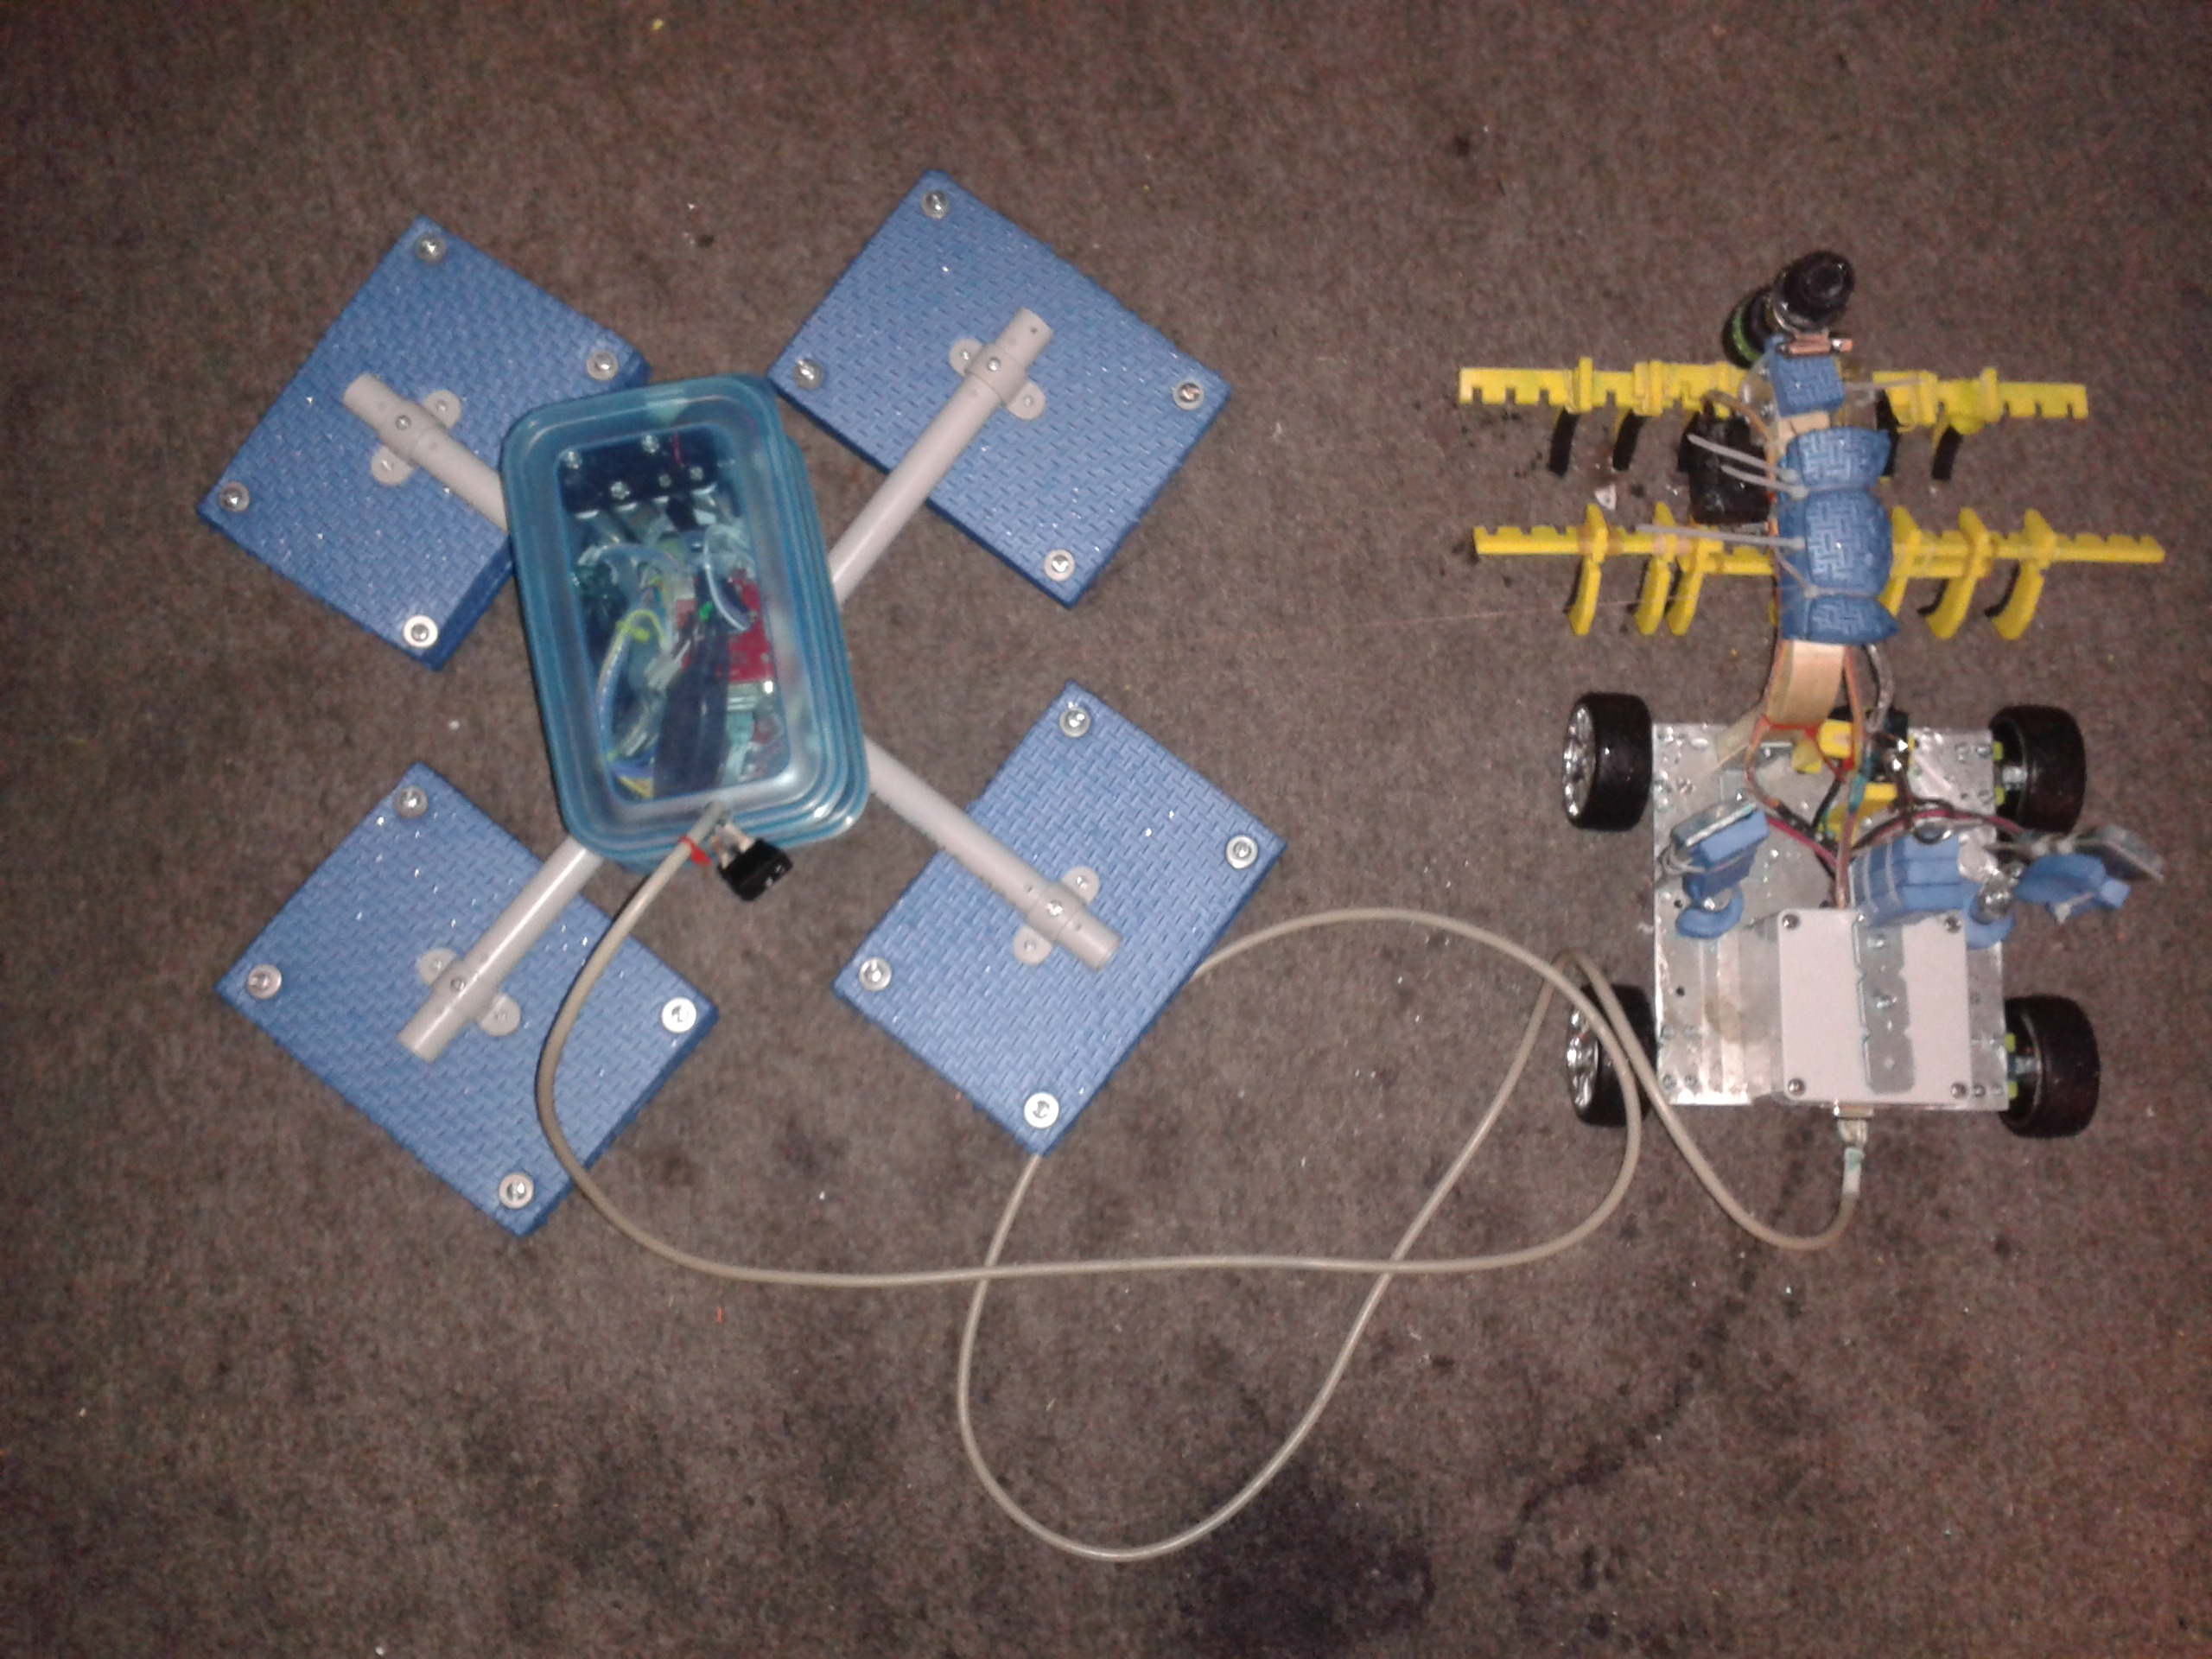
\includegraphics[width=0.7\textwidth]{20170529_053543}
\end{figure}


\section{System description}
The Goldfish consists of a buoy floating on the sea surface and a rover equipped with a camera and a claw. The Goldfish is controlled using a computer keyboard. Table \ref{tab:components} gives the complete list of parts that compose the Goldfish.
\begin{table}[H]
\begin{center}
\caption{List of parts composing the Goldfish.}
\label{tab:components}
\vspace{0.5cm}
\begin{tabular}{|c|c|}
\hline
\textbf{Part} & \textbf{Quantity}\\
\hline
Claw with arm & 1\\
\hline
Claw fingers & 11\\
\hline
Claw short finger & 1\\
\hline
Rover body & 1\\
\hline
Rover wheels & 4\\
\hline
DB cable & 1\\
\hline
Camera receiver & 1\\
\hline
Buoy arm & 4\\
\hline
Buoy foam & 4\\
\hline
Buoy electronic container & 1\\
\hline
Winch container & 1\\
\hline

\hline


\end{tabular}
\end{center}
\end{table}
\section{Assembly}
In order to assemble the Goldfish you will need the following tools:
\begin{itemize}
\item Screw drive
\item Wrench
\end{itemize}
Follow the steps below to assemble the Goldfish:
\begin{itemize}
\item Attach the servo container at the bottom of the electronic container making sure that the stepper wire are going through the holes to the PCB in the electronic container.
\item Connect each one of the arms to one side on the bottom of the winch container.
\item Attach the servo arm to the rover body using M4 bolts and nuts.
\item Mount the wheels to the rover DC motors.
\item Build the two side of the claw using the fingers as shown in figure. Attach each side the one of the claw sides. Make sure that the short finger is on the section containing the servo and that the short brace from the servo side.

\begin{figure}[H]
  \caption{Goldfish claw.}
  \centering
    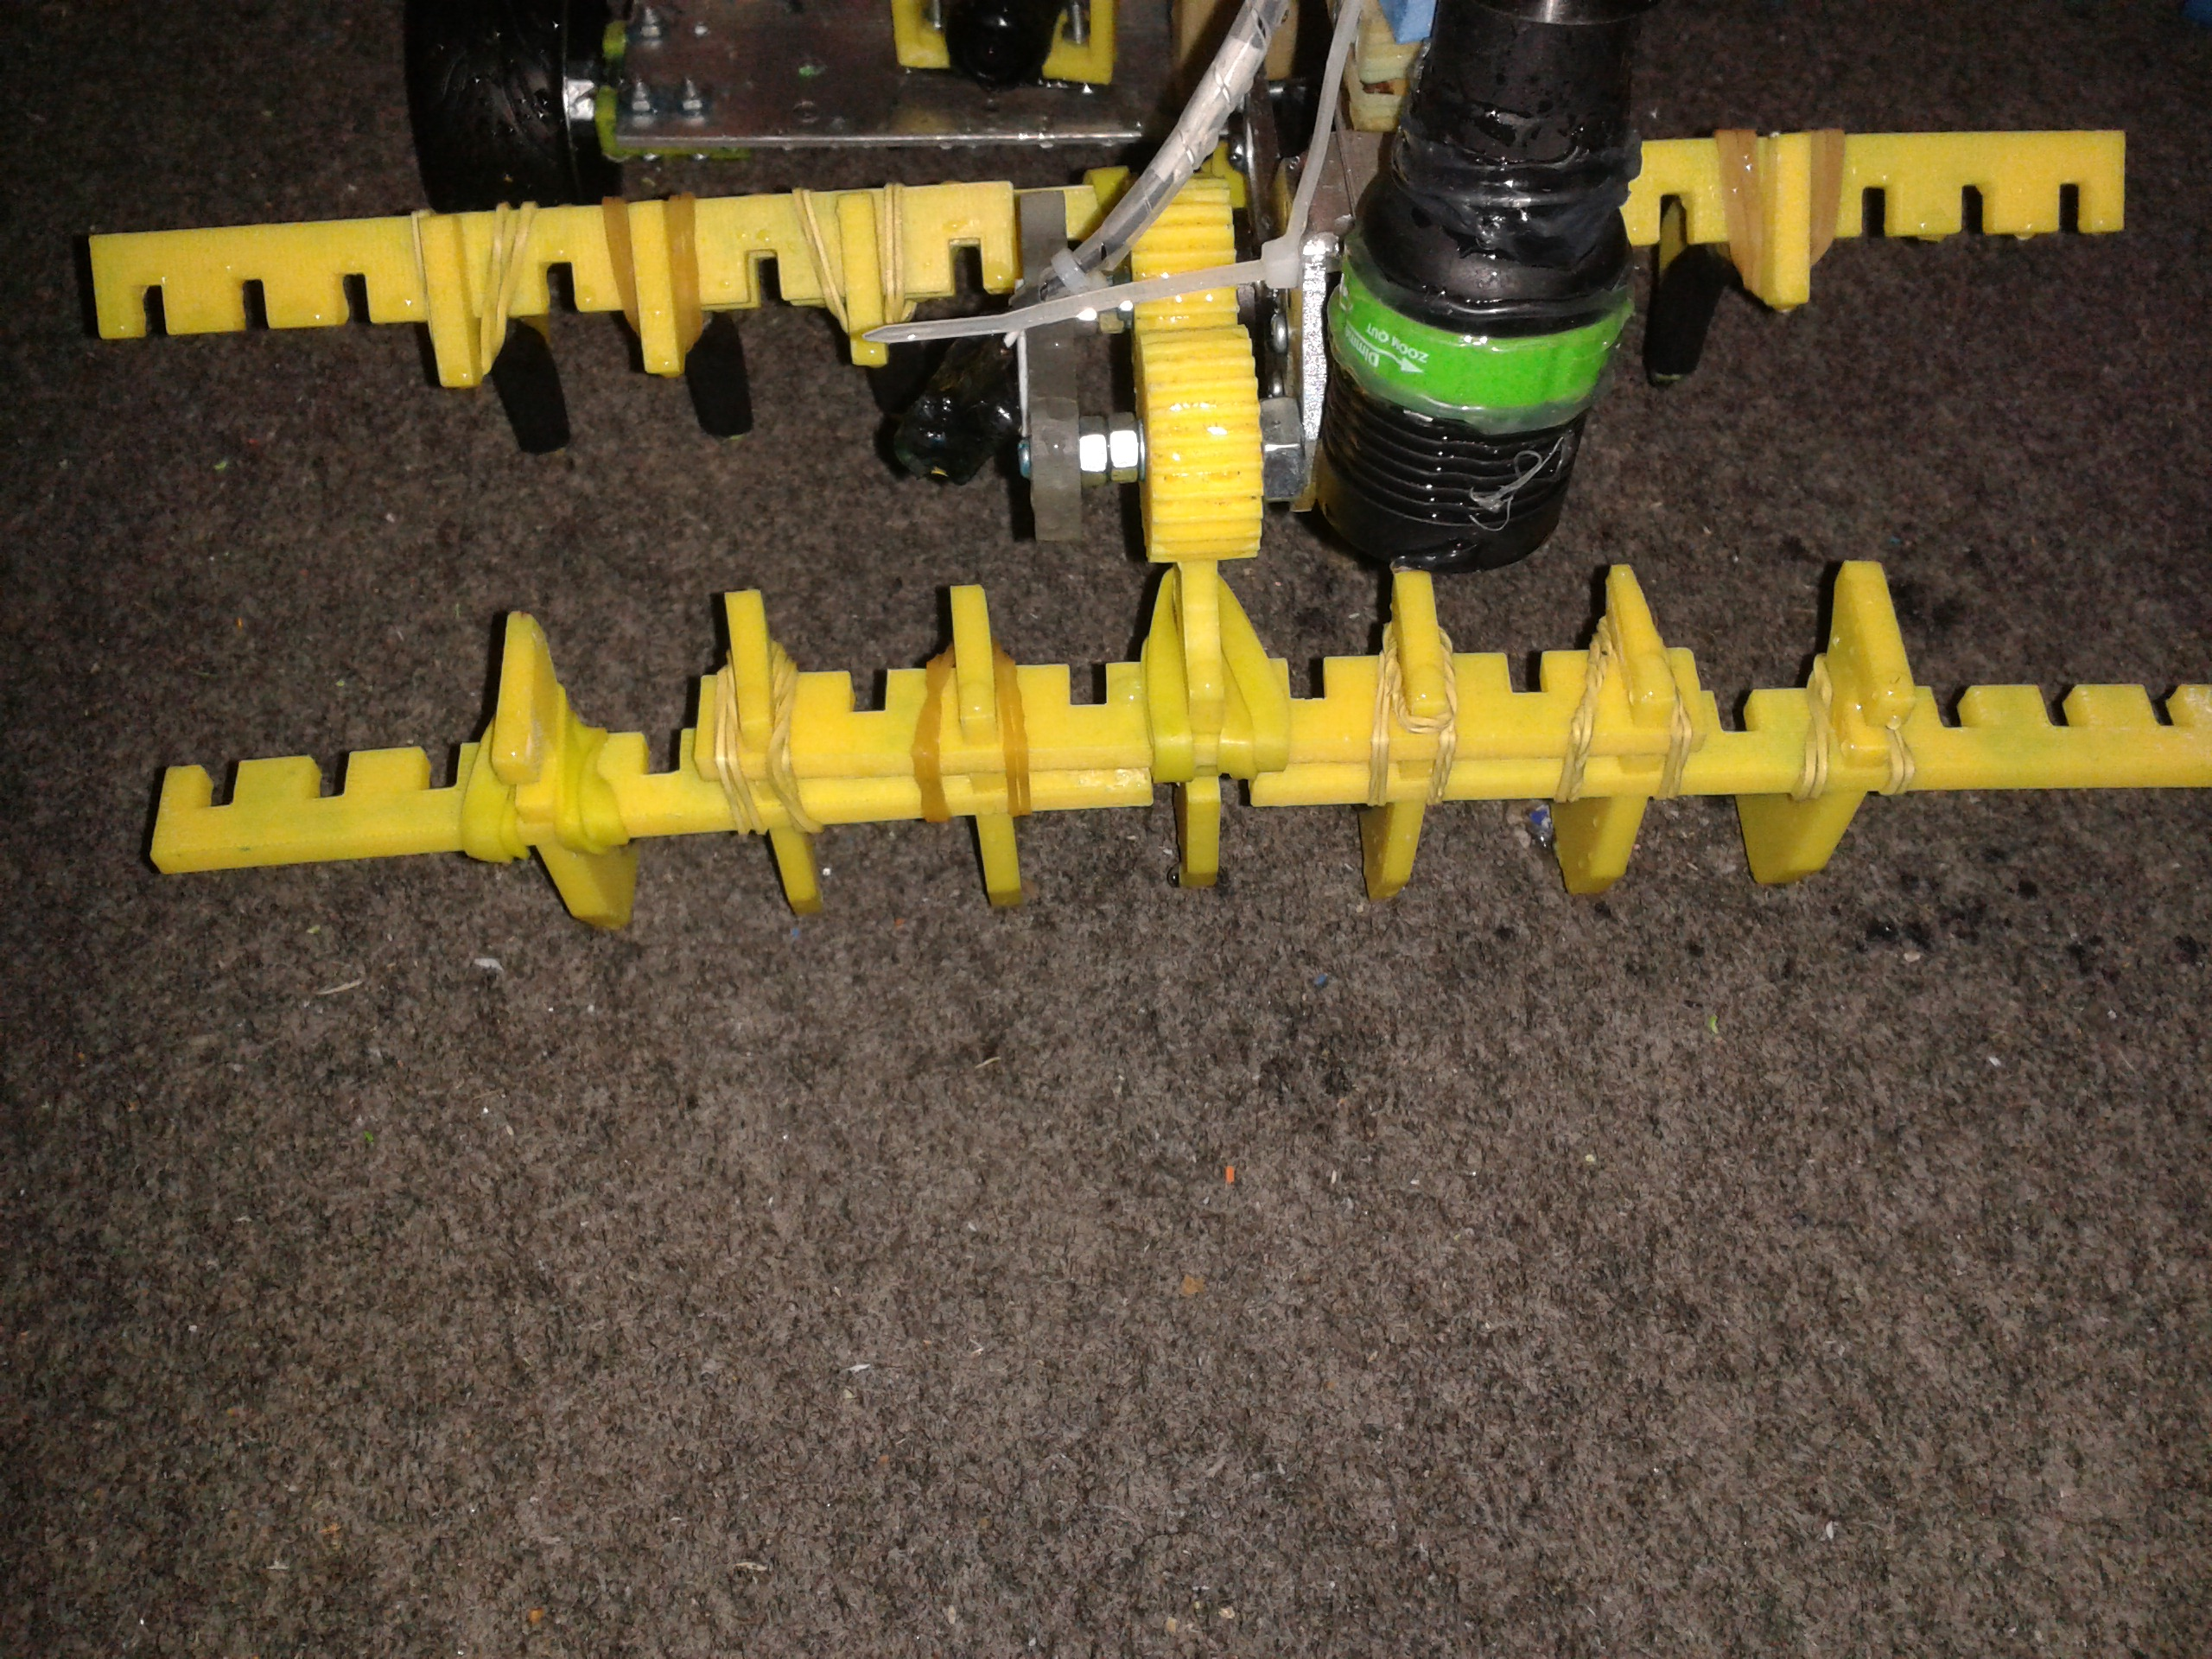
\includegraphics[width=0.6\textwidth]{20170529_053601}
\end{figure}
\end{itemize}
\section{Required software}
\subsection{Bluetooth communication}
The Goldfish is remotely controlled through bluetooth serial communication. After establishing the bluetooth connection with the Goldfish, you have several ways to communicate with the system. One possibility is to use the open source software PUTTY. PUTTY is an SSH and telnet client. To download and install PUTTY, use the following link. Select your platform and follow the instructions:
\url{https://www.chiark.greenend.org.uk/~sgtatham/putty/latest.html}.
\subsection{Camera software}
To run the Goldfish camera, you will need to download and install the open source software XSplit broadcaster using the following link:
\url{https://www.xsplit.com/#broadcaster}
\section{Starting the Goldfish}
To start the Goldfish, press the Start Button on the buoy.
\subsection{Starting the camera}
The camera receiver has to be connected to one of the computer USB ports. Then start XSplit. Once the XSplit is opened follow these steps:
\begin{itemize}
\item Click source in the menu bar.
\item Select Webcame,capture card, video devices.
\item Click AV TO USB2.0.
\end{itemize}
At that moment you should see the streaming from the camera. However the image is flipped. To correct it:
\begin{itemize}
\item Go to Scene at the bottom of the XSplit window.
\item Select AV TO USB2.0.
\item Click Settings on the bottom left of the XSplit window.
\item Select the tab Layout and the press flip horizontally.
\end{itemize}
\subsection{Establishing the bluetooth connection}
Establishing the Bluetooth models depends on the used platform, please refer to your platform bluetooth documentation. Here is a description for Windows users. Once the Goldfish is powered, in the computer under the Bluetooth properties, select "Add a device". The default device name of the Bluetooth module is "Goldfish". Double click "Goldfish" and select the "Hardware" tab, you can see which COM port the module is connected.
\subsection{Using serial communication}
As stated above, you may use any terminal programs for the serial communication. Here are the instruction for using PUTTY.
\begin{itemize}
\item Select the ‘Serial’ radio button.
\item Type the COM port number that the Bluetooth device is connecting to.
\item Set the default baud rate to 9600.
\item Click "Open". A terminal should be opened. The first line should contain the "Ready!" message which indicates that the Bad Bit is ready for receiving commands.
\end{itemize}
\section{System control}
The Goldfish is controlled through the keyboard. Table \ref{tab:keys} summarizes the keys that control the Goldfish. After pressing a key, it is not required to press the enter key. Once the command has been executed, a feedback message is displayed in the terminal followed by the current status of all actuators.
\begin{table}[h]
\begin{center}
\caption{Keys controlling the system.}
\label{tab:keys}
\vspace{0.5cm}
\begin{tabular}{|c|c|}
\hline
\textbf{Character} & \textbf{Action}\\
\hline
'q' & Move the winch rope up\\
\hline
'a' & Move the winch rope down\\
\hline
'x' & Hold the winch\\
\hline
'z' & Release the winch\\
\hline 
'w' & Move the claw servo 5$^{\circ}$ toward closing\\
\hline  
's' & Move the claw servo 5$^{\circ}$ toward opening\\
\hline
'e' & Move the camera servo 5$^{\circ}$ to the left\\
\hline  
'r' & Move the camera servo 5$^{\circ}$ to the right\\
\hline
'i' & Move the rover forward\\
\hline
'm' & Move the rover backward\\
\hline
'k' or space & Stop the rover\\
\hline
'l' & Turn the rover to the right\\
\hline
'j' & Turn the rover to the left\\
\hline

\end{tabular}
\end{center}
\end{table}
% -------------------------------------------------------------------------------------
% REFERENCES
% -------------------------------------------------------------------------------------
%\bibliography{}

% -------------------------------------------------------------------------------------
% END DOCUMENT
% -------------------------------------------------------------------------------------
\end{document}